The disturbance is now added to our SIMULINK model (see figure \ref{fig:linearModelNoise}).

\begin{figure}[H]
 \centering 
 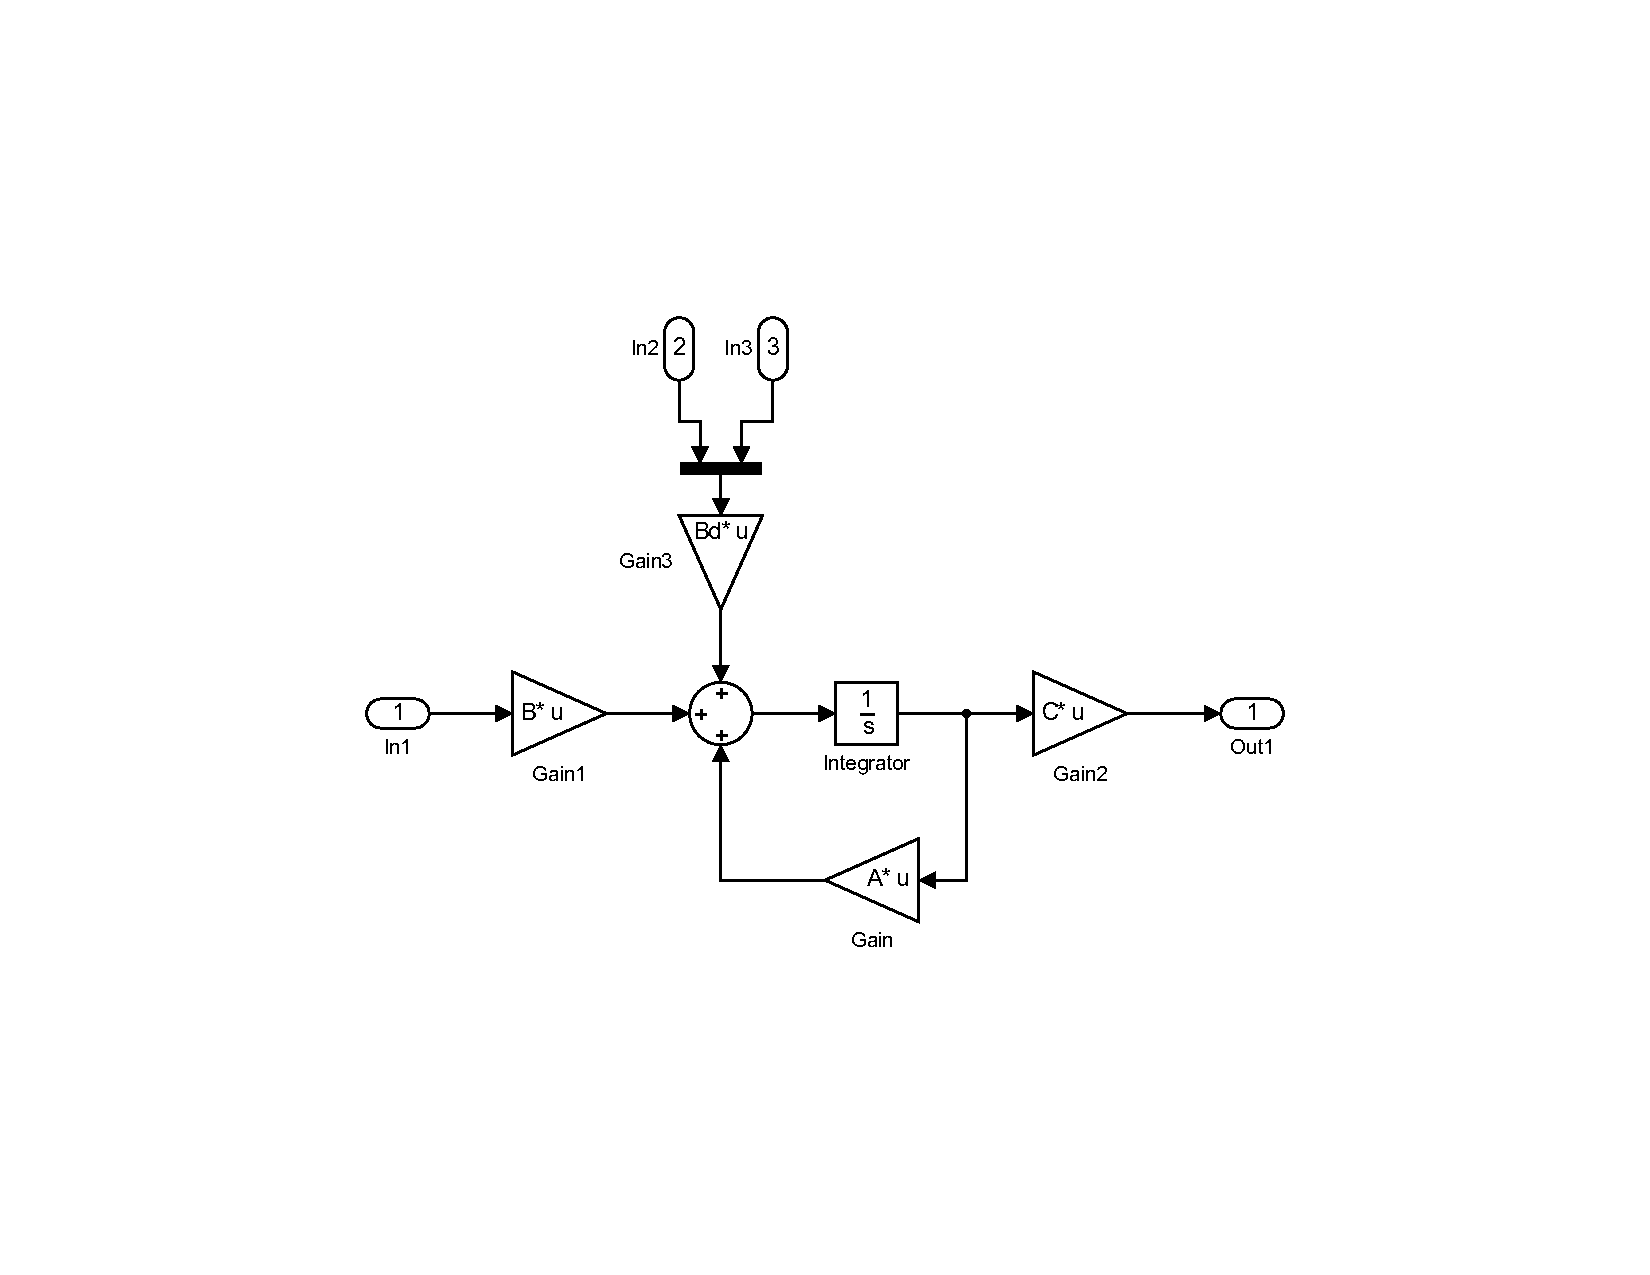
\includegraphics[trim=5cm 5cm 2cm 5cm, clip=true, totalheight=0.35\textheight, angle=0]{figures/linearModelNoise.pdf}
 \caption{SIMULINK model of the linearised loudspeaker with noise}
\label{fig:linearModelNoise}
\end{figure}

The response to the input can be seen figure \ref{fig:responseNoiset} and the PSD figure \ref{fig:responseNoisef}.

\begin{figure}[H]
 \centering 
 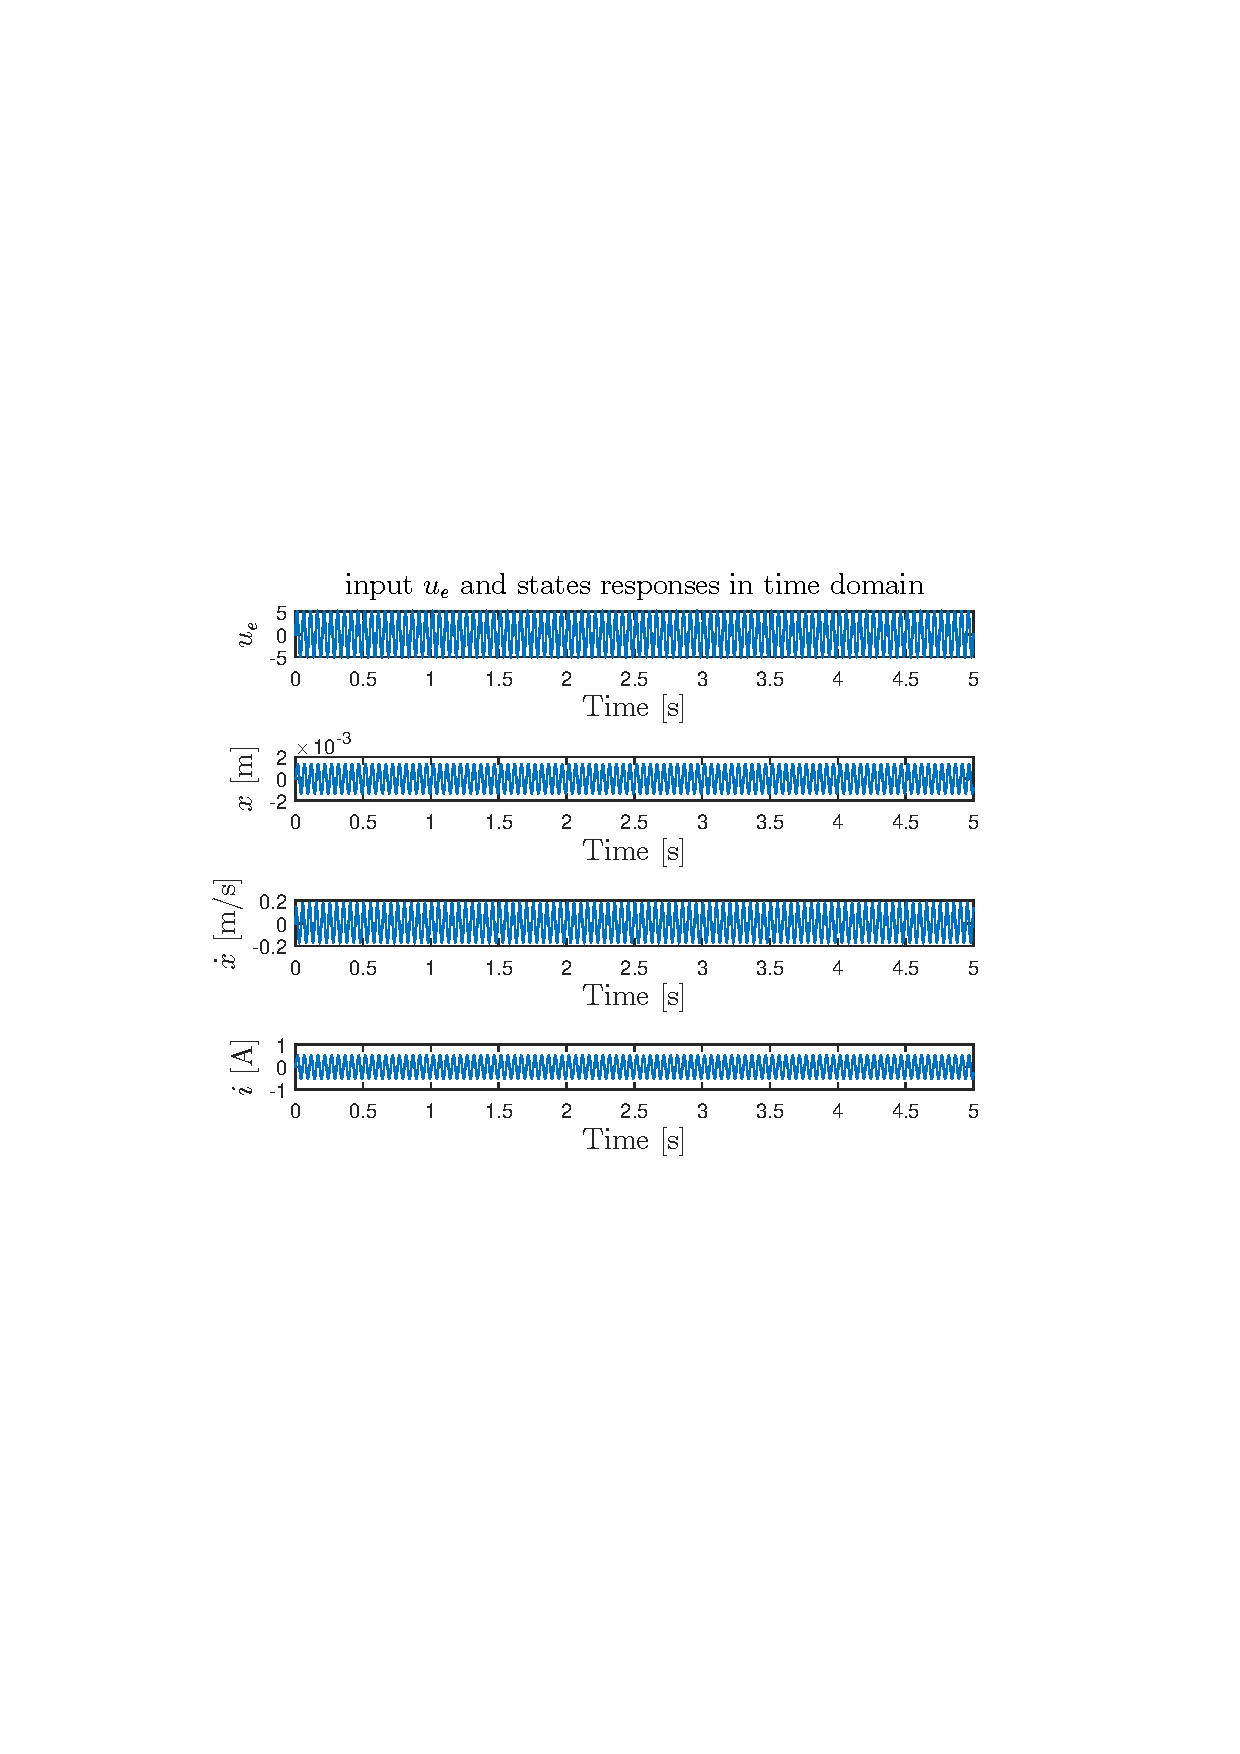
\includegraphics[trim=2cm 7cm 2cm 7cm, clip=true, totalheight=0.35\textheight, angle=0]{figures/responseNoiset.pdf}
 \caption{$u_e$ and states response to the input $u_e$ using the linearised model extended with disturbances}
 \label{fig:responseNoiset}
\end{figure}

\begin{figure}[H]
 \centering 
 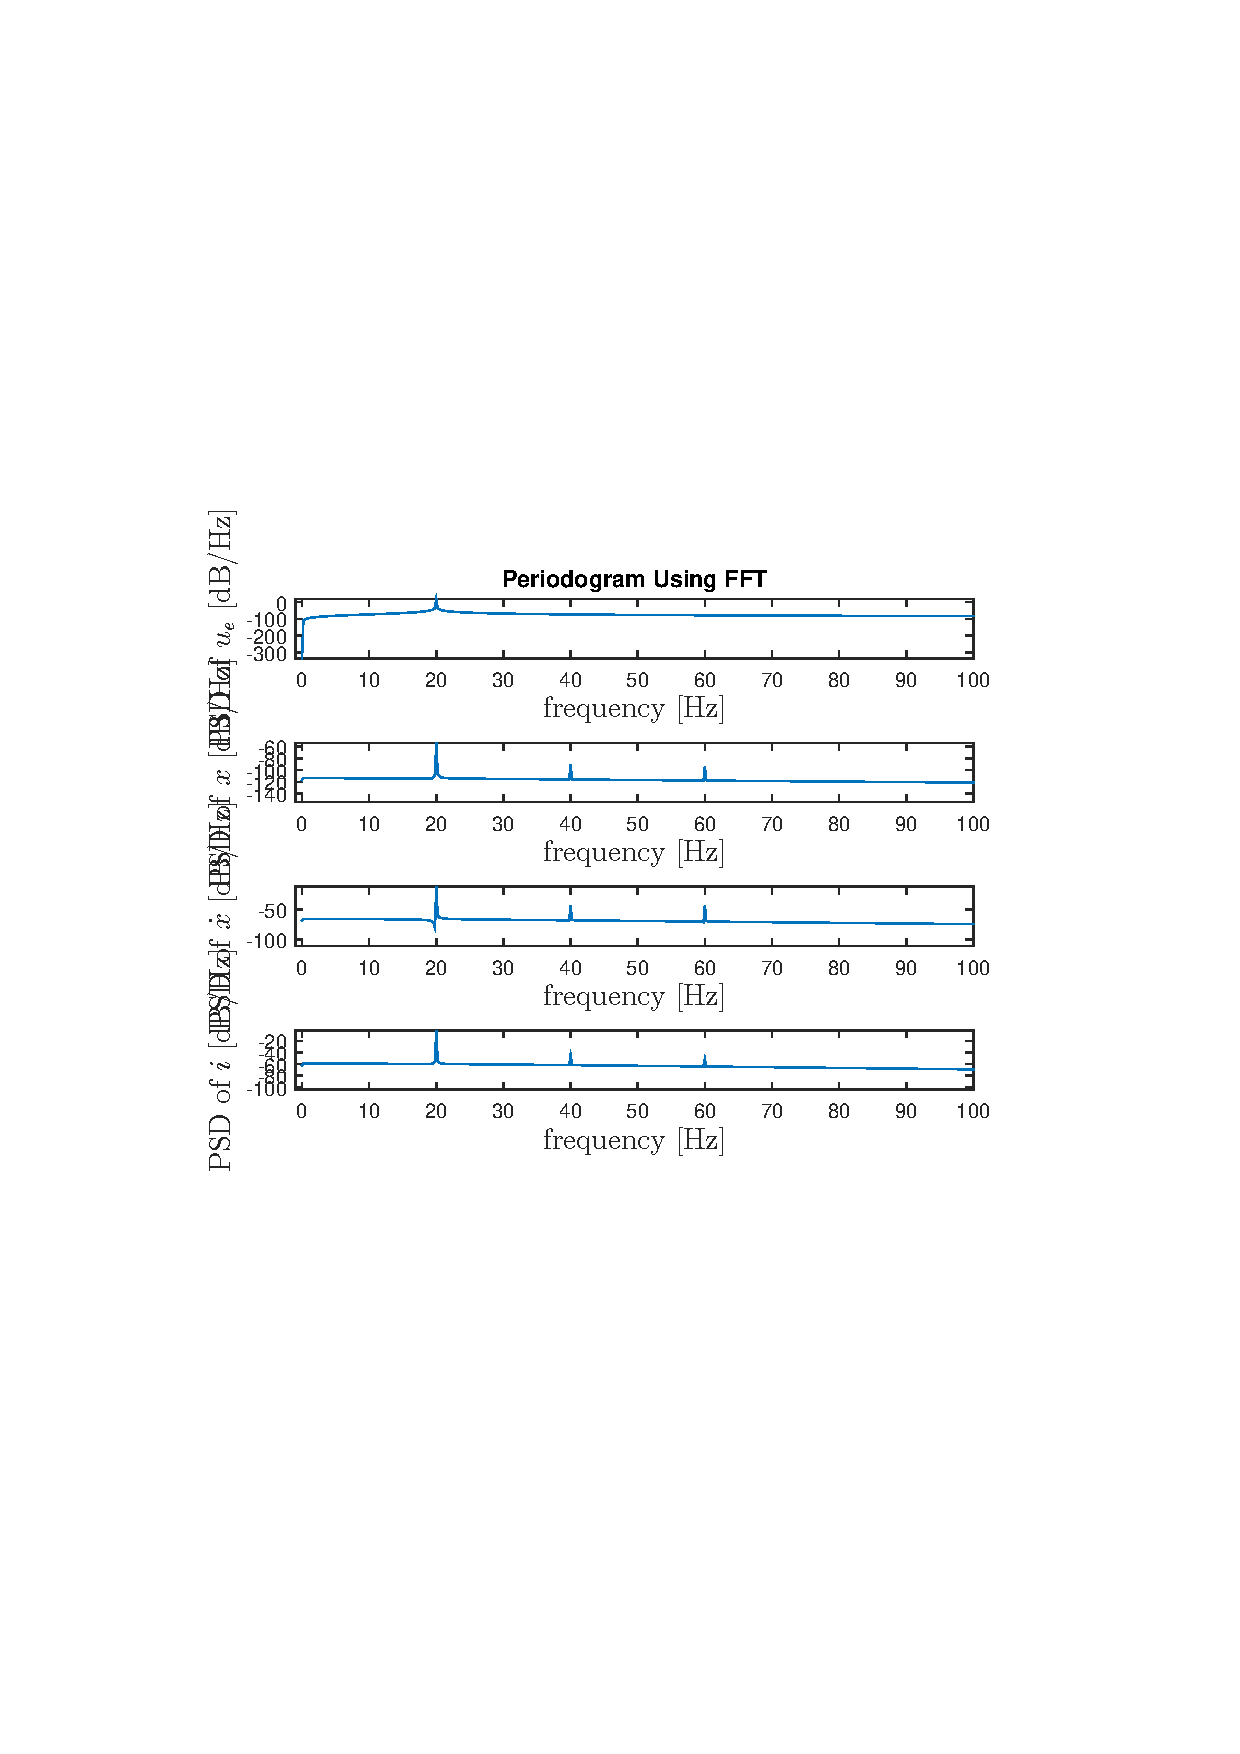
\includegraphics[trim=2cm 7cm 2cm 7cm, clip=true, totalheight=0.35\textheight, angle=0]{figures/responseNoisef.pdf}
 \caption{PSD of $u_e$ and states using the linearised model extended with disturbances}
 \label{fig:responseNoisef}
\end{figure}

We can see that the output of the new model permits to have the harmonic distortion at $f = 40$ and $60$ $Hz$ desired. However, we can notice that there is a difference of 2 $db$ for the third harmonic on the PSD figure \ref{fig:responseNoisef}. Therefore, we will reduce 'manually' the magnitude $A_{i2}$ to 0.075 $V$ in order to delete this error and improve the model.

